% !TEX root = ../diploma.tex

\section{Имя раздела работы}

\subsection{Зависимости}
Для начала разберемся, как это запускать. 

Нужен текстовый редактор. Можно использовать спец. программу, например, \texttt{TeXStudio}. 

Нужен компилятор \texttt{XeLaTeX} и система управлением библиографии \texttt{biber}. Все они включены в пакетах \texttt{MikTeX}/\texttt{TeXLive}. Если вы делаете частичную установку, то убедитесь, что выбрали необходимые пакеты. 

Если вы используете \texttt{Linux}, то просто скачиваете из ваших репозиториев \texttt{TeXLive}, и все готово. Может оказаться, что \texttt{biber} будет отдельным пакетом. 

В случае ошибок, связанных с отсутствием пакетов, просто доустановите их.

\subsection{Настройка \texttt{TeXStudio}}

Для начала нужно зайти в настройки и выбрать нужный компилятор для текста и библиографии. Делается это на вкладке Build. Нас интересует \texttt{XeLaTeX} и \texttt{Biber}.
\begin{figure}[H]
    \centering
    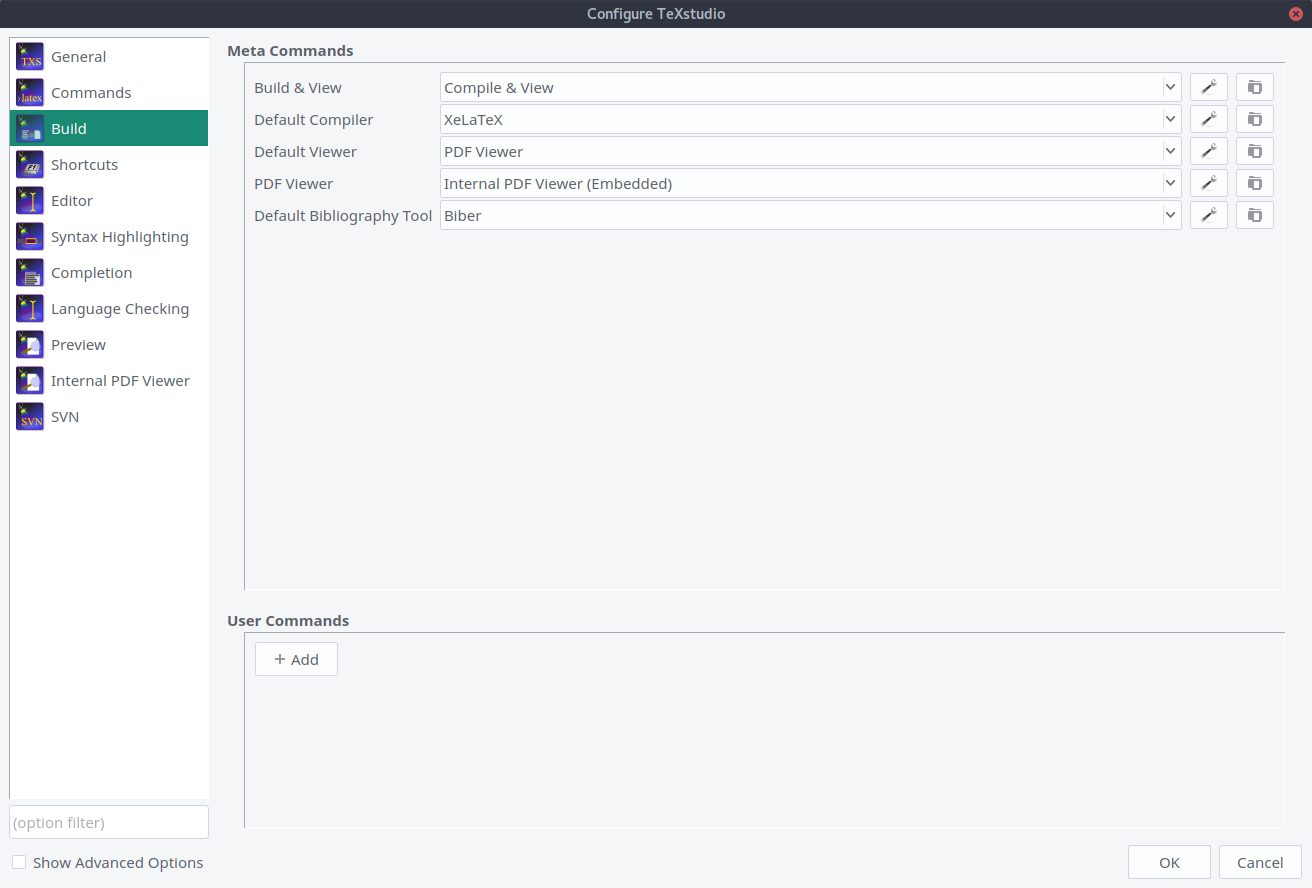
\includegraphics[keepaspectratio,width=0.5\textwidth]{settings}
\end{figure}


\subsection{Ошибки при работе с \LaTeX}
Если при сборке библиография не появилась -- не пугайтесь. \texttt{biber} нужно запускать \textbf{отдельно}. В  это делается очень удобно: Tools $\rightarrow$ Bibliography (либо запустите его руками в терминале).

Если вдруг вместо ссылки на уравнение (или цитирование, или что-нибудь подобное) вы получаете имя самой метки -- просто запустите компиляцию второй раз. \LaTeX\, требует двух проходов для составления ссылок, оглавления и ряда других вещей. 


\subsection{Цитирование и ссылки}
Делать ссылки к библиографии -- это просто! Достаточно поставить \texttt{\\cite\{ссылка\}}. Ссылки не пишутся слитно, поэтому перед \texttt{cite} нужен пробел. Выглядит это примерно так \cite{test}.

Для уравнений можно использовать специальное окружение. Любые окружения (в т.ч. уравнения), можно помечать для дальнейшей возможности ссылки. Для этого используется \texttt{label}. Для уравнений есть специальная (совсем необязательная) версия: \texttt{label\{eq:имя\}} Пример:
\begin{equation}\label{eq:some_eq}
	e^2 = E\{(F - Y)^2\},
\end{equation}
где $E$ -- математическое ожидание.

Чтобы получить ссылку, достаточно вставить макрос \texttt{ref\{имя\}}. Для уравнений (в случае использования специальной версии) есть \texttt{eqref}. Получим следующее: \eqref{eq:some_eq}.

\subsection{Списки}
Иногда хочется сжать список. Чтобы не настраивать интервал между списками (это делается не очень удобно) достаточно передать параметр \texttt{[noitemsep]}.

Без сжатия:
\begin{itemize}
    \item пункт 1
    \item пункт 2
\end{itemize}

С сжатием:
\begin{itemize}[noitemsep]
    \item пункт 1
    \item пункт 2
\end{itemize}

\subsection{Код и псевдокод}
Вставить код тоже просто. Если настройки листинга не устраивают, то с ними можно поиграться. Макрос настройки находится в файле \texttt{packages}.

\begin{lstlisting}[caption={Пример вызова БПФ в библиотеке \texttt{CuFFT}}]
	cufftComplex *d_signal;
	cudaMalloc((void **) &d_signal, mem_size); 
	cudaMemcpy(d_signal, fg, mem_size, cudaMemcpyHostToDevice);
	
	cufftHandle plan;
	cufftPlan2d(&plan, N, N, CUFFT_C2C);
	
	cufftExecC2C(plan, (cufftComplex *)d_signal, (cufftComplex *)d_signal, CUFFT_FORWARD);
\end{lstlisting}

Также можно писать псевдокод. Ключевые слова можно переводить, вводить новые конструкции и т.д. Пример в файле \texttt{commands}.
\begin{algorithm}
    \caption{Пример псевдокода}
    \begin{algorithmic}[1] % The number tells where the line numbering should start
        \Procedure{F}{$A$, $B$, $N$}
        \State $E \gets A$
        \For{$i := 1$ до $N$}
        \State $\hat{E} = \texttt{fft}~E$
        \State $\hat{I} = \hat{E}\times \hat{H}$
        \EndFor
        \State \textbf{вернуть} $E$
        \EndProcedure
    \end{algorithmic}
\end{algorithm}

\subsection{Таблицы}
Здесь используется вспомогательное окружение \texttt{tabularx} (есть "брат" -- \texttt{tabulary}), которое управляет шириной столбцов и автоматически переносит текст на новую строку в той же ячейке при нехватке размерности.

\begin{table}[H]
	\centering
	\begin{tabularx}{\textwidth}{| X | X | X |}
		\hline
		\textbf{Размер изображения} & \textbf{Время GPU} & \textbf{Время CPU} \\ \hline
		$1920\times 1920$           & 6 мс               & 75 мс              \\ \hline
		$4096\times 4096$           & 24 мс              & 520 мс             \\ \hline
		$3648\times 5472$           & 35 мс              & 625 мс             \\ \hline
	\end{tabularx}
	\caption{Сравнение скорости работы}
\end{table}

\subsection{Фигуры}
В окружение \texttt{figure} можно помещать обычный \texttt{includegraphics}, таблицы, элементы \texttt{tikz}, создавать массивы изображений и т.д. 

\paragraph{Пример массива изображений.}
Подписи не являются обязательными. Нумерация \texttt{subfloat}'ов можно выключить в \texttt{captionsetup}. Там же набор других настроек внешнего вида подписей.

Для задания расстояния между картинками использовать стандартные макросы шага, т.е. \texttt{quad, qquad} и т.д.

Если картинки нет, но прикинуть внешний вид и подобрать размер хочется, то можно использовать стандартные \texttt{example-image-[a,b,c]}.

\begin{figure}[H]
	\centering
	\captionsetup[subfigure]{justification=centering}
	\subfloat[Пример]{\includegraphics[height=0.1\textwidth]{example-image-a}}%
	\quad
	\subfloat[Пример]{\includegraphics[height=0.2\textwidth]{example-image-b}}%
	\quad
	\subfloat[Пример]{\includegraphics[height=0.1\textwidth]{example-image-c}}%
	\quad
	\subfloat[Очень длинная подпись, которая перенесется на новую строку]{\includegraphics[height=0.15\textwidth]{example-image-a}}%
	\caption{Общая подпись к фигуре}
\end{figure}
